\documentclass{standalone}

\usepackage{pgfplots}

\usepgfplotslibrary{fillbetween}

\begin{document}

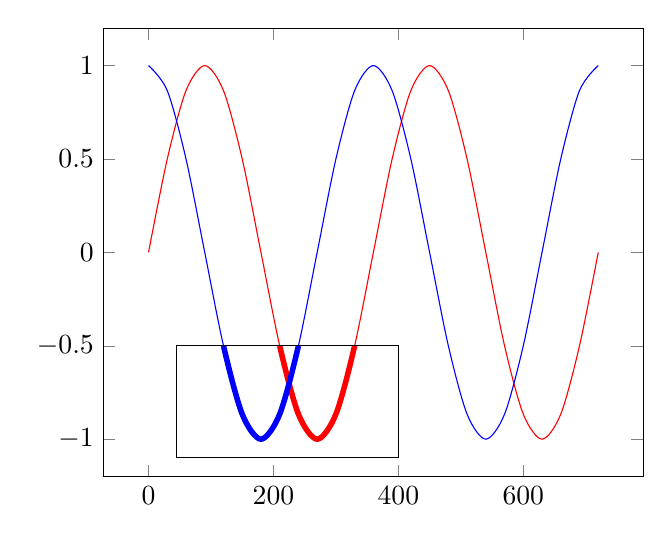
\begin{tikzpicture}
%\def\pgfintersectiontolerance{2pt}
	\begin{axis}[domain=0:720,samples=25,smooth
		]
	\def\clippath{(axis cs:45,-1.1) rectangle (axis cs:400,-0.5)
	}
	\addplot[red,name path=A,
		postaction={decorate,line width=2pt,
			decoration={soft clip,
				soft clip path=\clippath
			},
		},
	] {sin(x)};

	\addplot[blue,name path=B,
		postaction={decorate,line width=2pt,
			decoration={soft clip,
				soft clip path=\clippath
			},
		},
	] {cos(x)};

	\addplot fill between[of = A and B,
		soft clip={\clippath},
	];

	\draw \clippath;
	\end{axis}
\end{tikzpicture}
\end{document}

